\chapter{Urban Source Identification Results and Discussion}

% Compare how well we identify shielded/unshielded isotopes when training set has shielding, doesn't have shielding. 

% Compare how well we identify isotopes over different distances if training set has one vs many distances

% Compare how well we identify isotopes with different calibration sampling granularity 

% https://e-reports-ext.llnl.gov/pdf/312592.pdf holy shit they show common false positive isotopes and we see a lot of overlap



\section{Problem Description and Training Dataset Overview}

This chapter applies machine learning algorithms to solve the problem of a identifying a radioactive source in an urban environment where a source may be present. This scenario is applicable when performing source interdiction searching cargo containers, vehicles at boarder crossings, or security at high profile events. Urban environments present unique challenges to gamma-ray spectroscopy. Background radiation can change over city blocks due to different concentrations of uranium and thorium in building materials. Sources may be purposely shielded by unknown amounts of material to obscure their gamma-ray signal.





\section{Online Data Augmentation Method}

Because simulating a dataset with sufficient combinations of available data augmentation - seen in Tables \ref{table:all_fixed_simulation_parameters} and \ref{table:all_variable_simulation_parameters} - online data augmentation techniques are employed. Online data augmentation has the benefit of implicitly regularizing the models.

Steps in the data augmentation process are:
\begin{enumerate}
  \item Randomly choose a background template with the same FWHM as the source template
  \item Rebin source and background template with a random calibration
  \item Apply the LLD to both templates
  \item Normalize both templates by the sum of their respective counts 
  \item Scale both signals by their respective total counts
  \begin{itemize}
     \item Counts defined by randomly chosen background counts per second, integration time, and signal to background ratio
   \end{itemize}
  \item Add both signals 
  \item Poisson sample the resulting signal
\end{enumerate}


\section{Learning Curve Comparison for Fixed-size Datasets and Online Data Augmentation Datasets}

In this section we use learning curves to quantify how well the online data augmentation improved testing error. Learning curves are [definition, explanation]. Learning curves are used to determine a few things. We will use them to do [the following].

First, They are used as a sanity check, to make sure we are sampling our input space with enough granularity. To know we are sampling well enough, we should be sampling in a region where the curves are flat for both algorithms.

Secondly, Learning curves give us insight into which algorithm works better on the hyperparameter optimization dataset and simple version of the problem. We're expecting the CNN to outperform the DNN due to theoretical benefits of convolution architectures for our problem. We can also compare this curve to the final learning curves for the final datasets.


\begin{figure}[H]
	\centering
	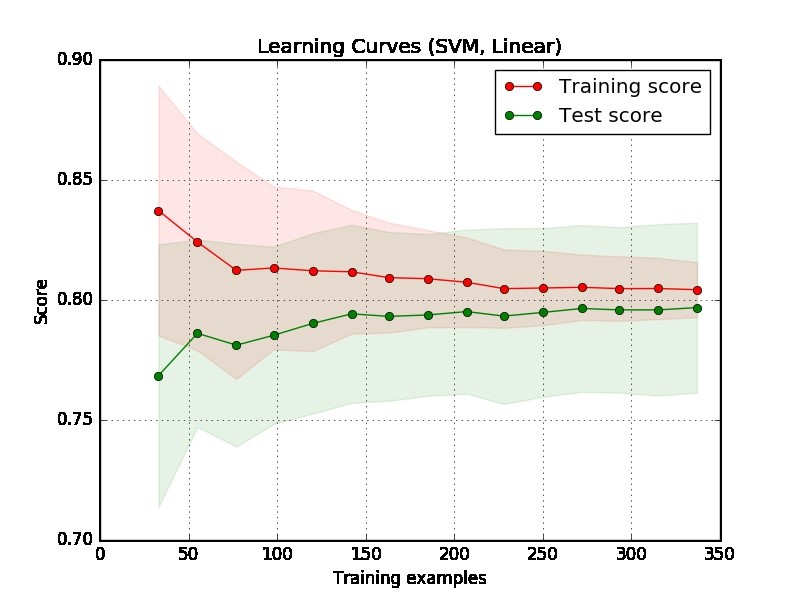
\includegraphics[width=0.8\linewidth]{model_choice_hyperparameter_search_images/learning_curve_dummy}
	\caption{Learning curves from the best DNN with best performance from online data augmentation. Shown: learning curve example.}
	\label{fig:learning_curves}
\end{figure}



\begin{figure}[H]
	\centering
	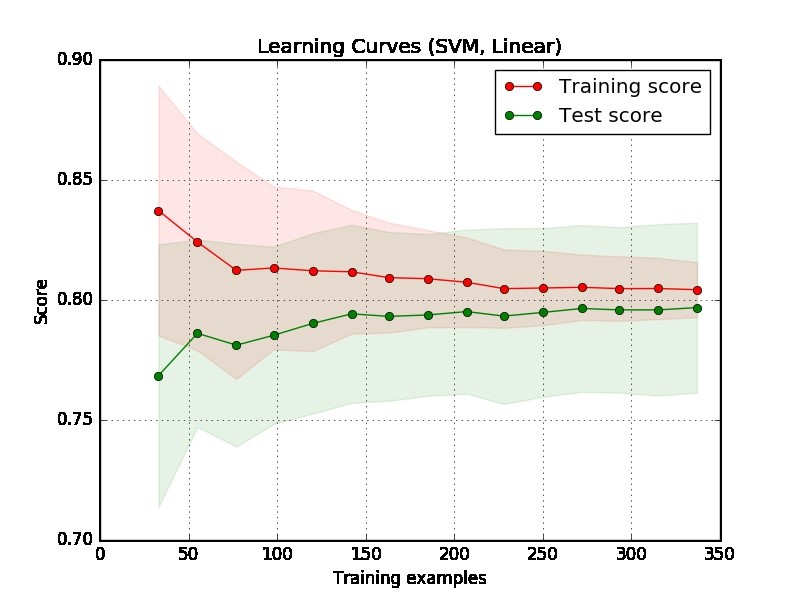
\includegraphics[width=0.8\linewidth]{model_choice_hyperparameter_search_images/learning_curve_dummy}
	\caption{Learning curves from the best CNN with best performance from online data augmentation. Shown: learning curve example.}
	\label{fig:learning_curves}
\end{figure}


\section{Generalization Performance Evaluation}

In this section we analyze the generalization performance of each network on various datasets. To quantify performance on a range of spectra qualities, the F1-scores are shown over integration time and for different signal to background ratios. When the error between models differs significantly or is particularly large, confusion matrices are included to show what isotopes are problematic.

Could also change the underlying distribution away from the training set by simulating a new template dataset with a different clutter parameter.

A default dataset will be modified. The default dataset will be  correspond to unshielded templates. 

\subsection{Generalization Performance on Source-Detector Distance and Height Off Ground}

In this section we analyze the generalization performance of each network on changes in source-detector distance and height. This tests if each model is sensitive to changes in the Compton continuum due to environmental scattering. Good performance in these simulated data may indicate better performance in real data.

To test generalization performance, datasets are simulated with unshieled spectral templates with a FWHM of 7.5. 


\begin{figure}[H]
     \centering
     \begin{subfigure}[b]{0.9\textwidth}
         \centering
         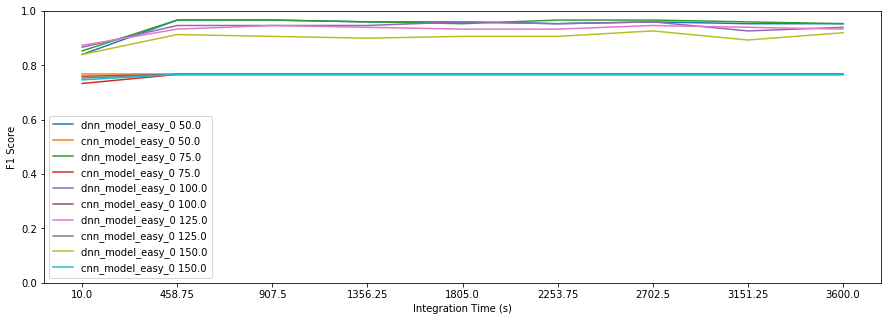
\includegraphics[width=\textwidth]{images/results_easy_distance_comparison}
         \caption{Simple Dataset.}
         \label{fig:results_easy_distance_comparison_simple}
     \end{subfigure}

     \begin{subfigure}[b]{0.9\textwidth}
         \centering
         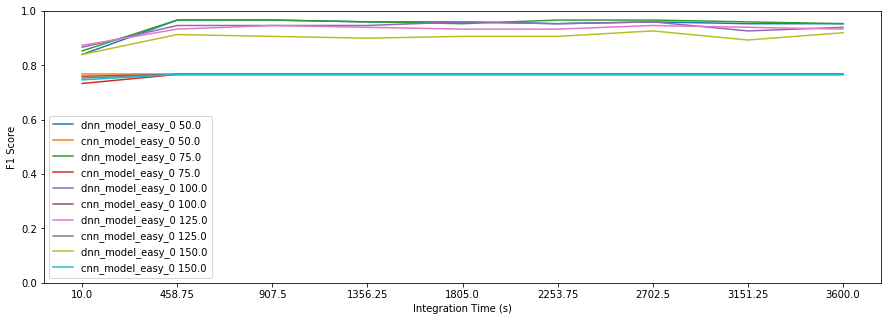
\includegraphics[width=\textwidth]{images/results_easy_distance_comparison}
         \caption{Full Dataset.}
         \label{fig:results_easy_distance_comparison_full}
     \end{subfigure}
        \caption{F1 score for all models trained on the simple dataset. Datasets included here used various source-detector distance.}
        \label{fig:results_easy_distance_comparison}
\end{figure}

\begin{figure}[H]
     \centering
     \begin{subfigure}[b]{0.9\textwidth}
         \centering
         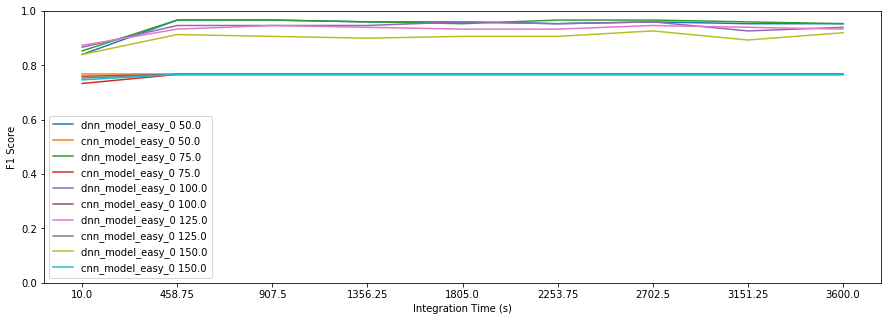
\includegraphics[width=\textwidth]{images/results_easy_distance_comparison}
         \caption{Simple Dataset.}
         \label{fig:results_easy_distance_comparison_simple}
     \end{subfigure}

     \begin{subfigure}[b]{0.9\textwidth}
         \centering
         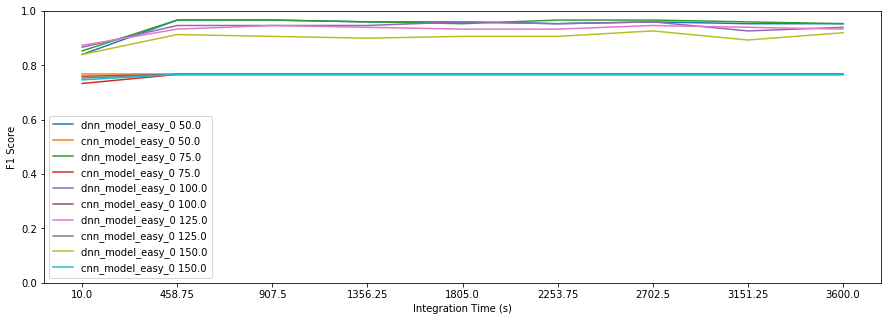
\includegraphics[width=\textwidth]{images/results_easy_distance_comparison}
         \caption{Full Dataset.}
         \label{fig:results_easy_distance_comparison_full}
     \end{subfigure}
        \caption{F1 score for all models trained on the simple dataset. Datasets included here used various source-detector heights.}
        \label{fig:results_easy_distance_comparison}
\end{figure}



\subsection{Generalization Dependence on Full-Width-at-Half-Max}

Datasets were constructed with various Gaussian energy broadening function. This is to 

\begin{figure}[H]
     \centering
     \begin{subfigure}[b]{0.9\textwidth}
         \centering
         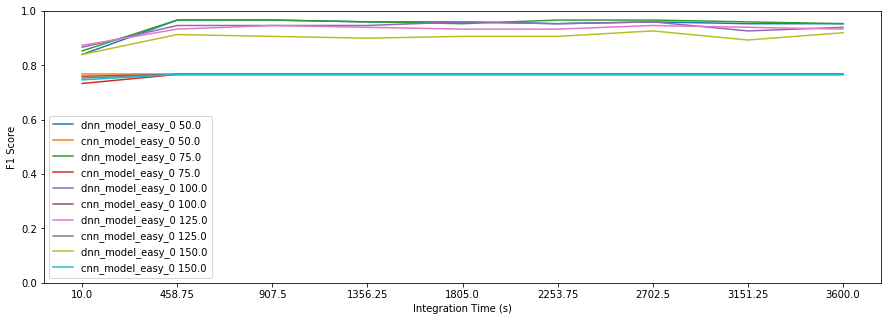
\includegraphics[width=\textwidth]{images/results_easy_distance_comparison}
         \caption{Simple Dataset.}
         \label{fig:results_easy_distance_comparison_simple}
     \end{subfigure}

     \begin{subfigure}[b]{0.9\textwidth}
         \centering
         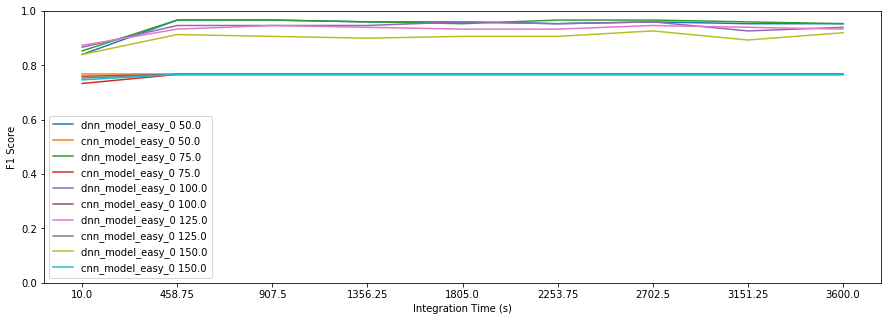
\includegraphics[width=\textwidth]{images/results_easy_distance_comparison}
         \caption{Full Dataset.}
         \label{fig:results_easy_distance_comparison_full}
     \end{subfigure}
        \caption{F1 score for all models trained on the simple dataset. Datasets included here used various Gaussian energy broadening functions.}
        \label{fig:results_easy_distance_comparison}
\end{figure}


\subsection{Generalization Dependence on Shielding.}

Datasets were simulated with and without shielding. 

\begin{figure}[H]
     \centering
     \begin{subfigure}[b]{0.9\textwidth}
         \centering
         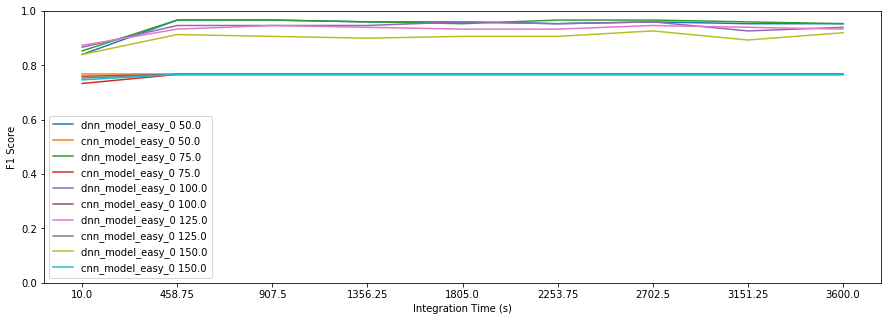
\includegraphics[width=\textwidth]{images/results_easy_distance_comparison}
         \caption{Simple Dataset.}
         \label{fig:results_easy_distance_comparison_simple}
     \end{subfigure}

     \begin{subfigure}[b]{0.9\textwidth}
         \centering
         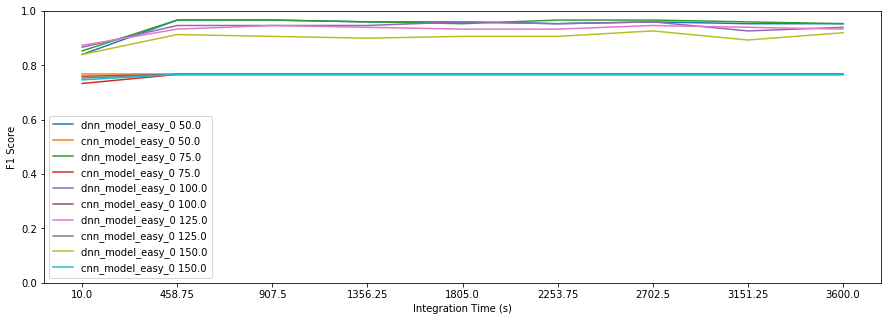
\includegraphics[width=\textwidth]{images/results_easy_distance_comparison}
         \caption{Full Dataset.}
         \label{fig:results_easy_distance_comparison_full}
     \end{subfigure}
        \caption{F1 score for all models trained on the simple dataset. Datasets included here used various amounts of shielding.}
        \label{fig:results_easy_distance_comparison}
\end{figure}


\begin{figure}[H]
     \centering
     \begin{subfigure}[b]{0.8\textwidth}
         \centering
         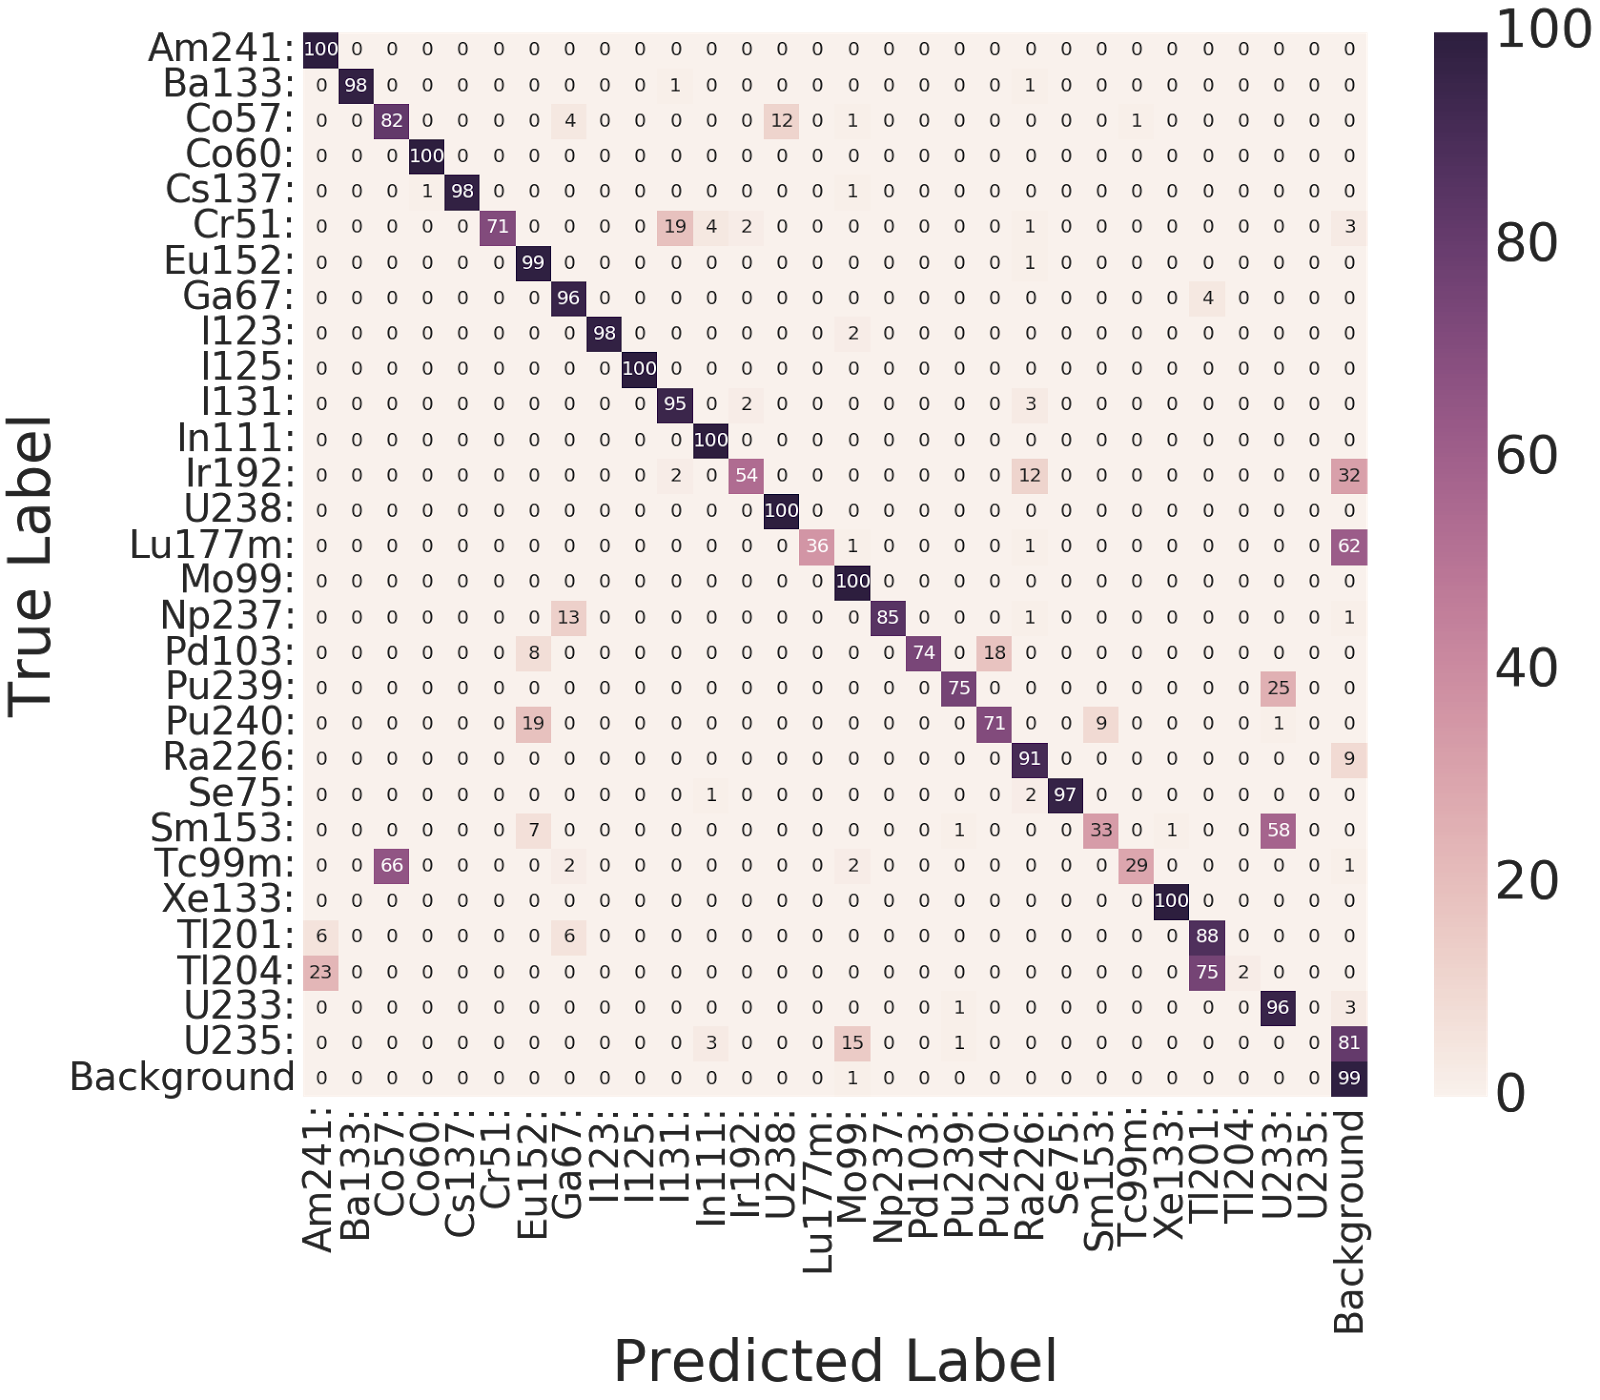
\includegraphics[width=\textwidth]{model_choice_hyperparameter_search_images/conf_matrix_example.png}
         \caption{Simple Training Dataset.}
         \label{fig:results_easy_distance_comparison_simple}
     \end{subfigure}

     \begin{subfigure}[b]{0.8\textwidth}
         \centering
         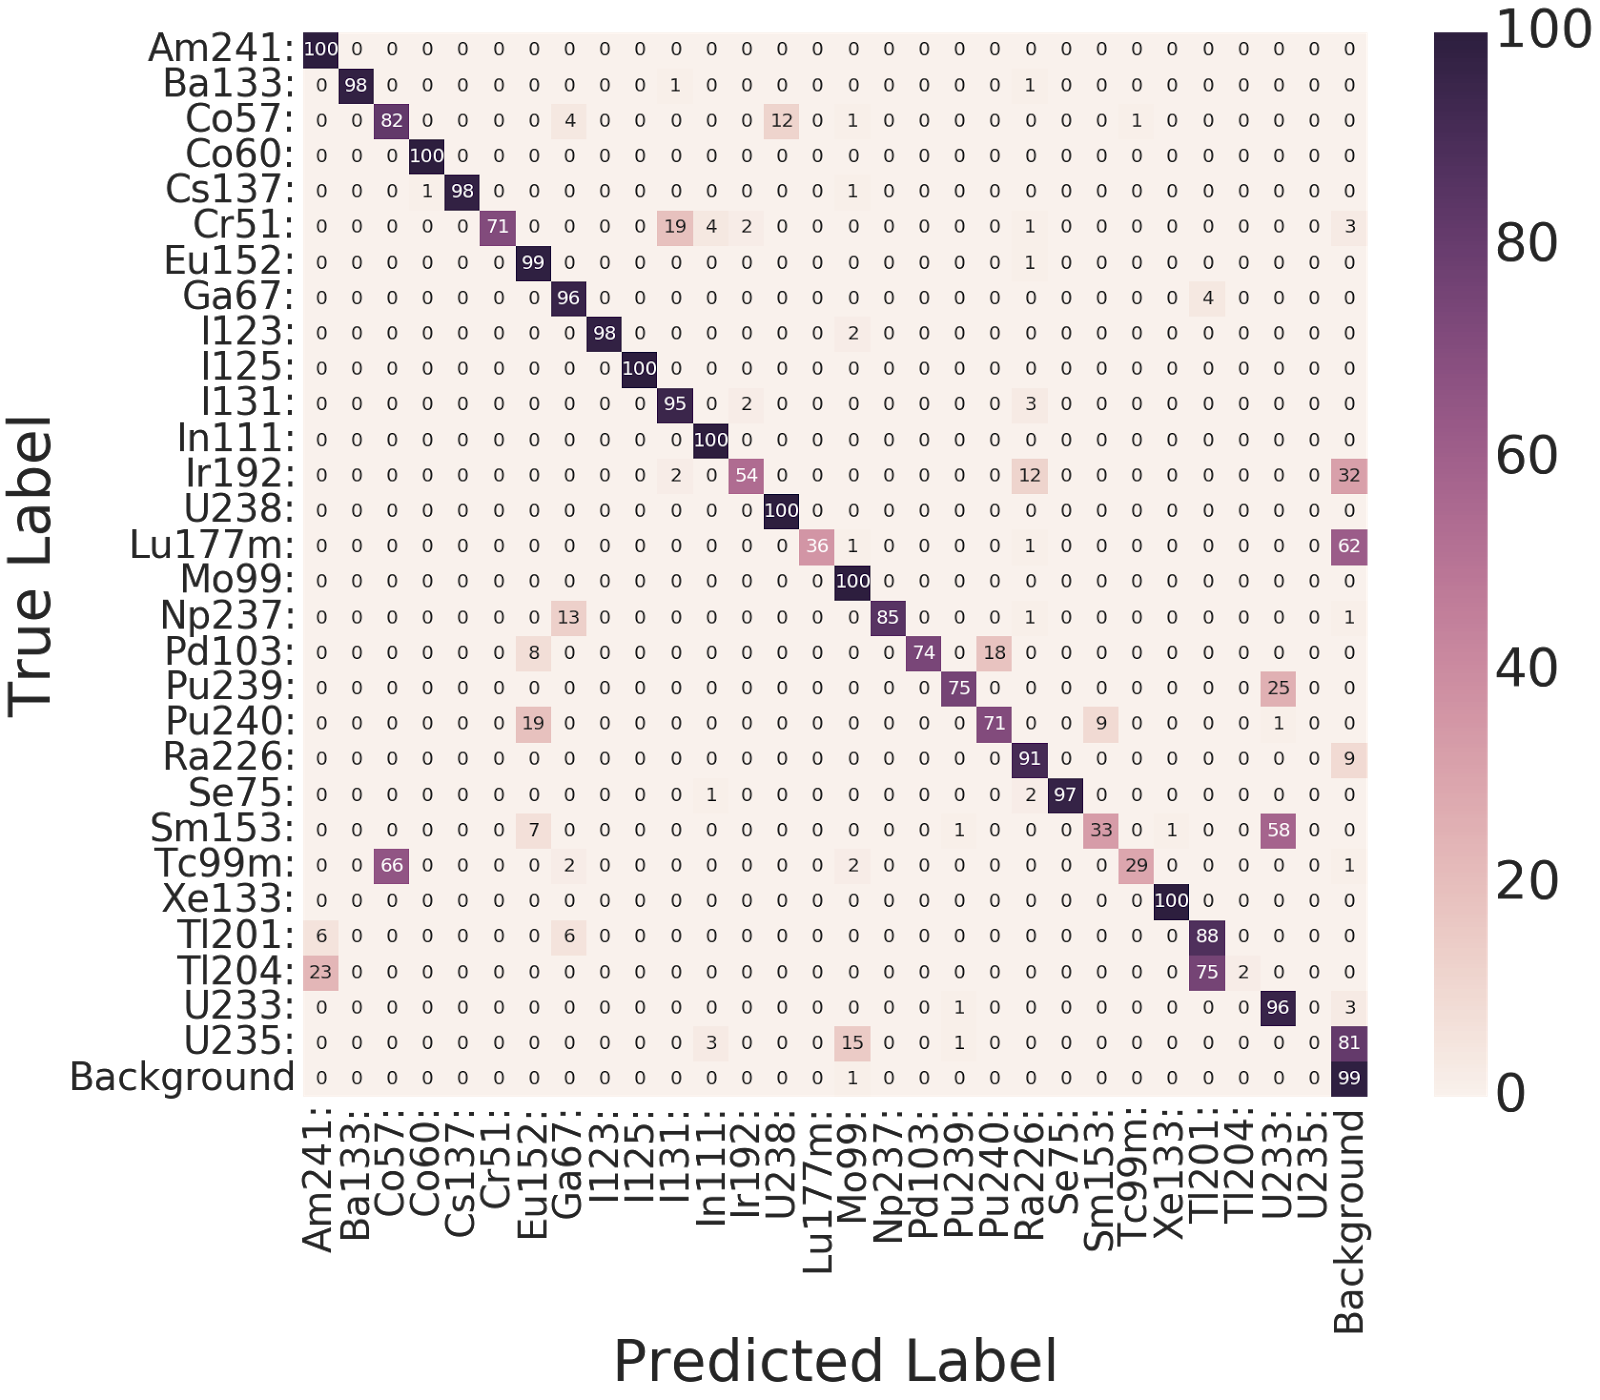
\includegraphics[width=\textwidth]{model_choice_hyperparameter_search_images/conf_matrix_example.png}
         \caption{Full Training Dataset.}
         \label{fig:results_easy_distance_comparison_full}
     \end{subfigure}
        \caption{Confusion matrices for the dataset with 60\% shielding.}
        \label{fig:results_easy_distance_comparison}
\end{figure}

\begin{figure}[H]
     \centering
     \begin{subfigure}[b]{0.49\textwidth}
         \centering
         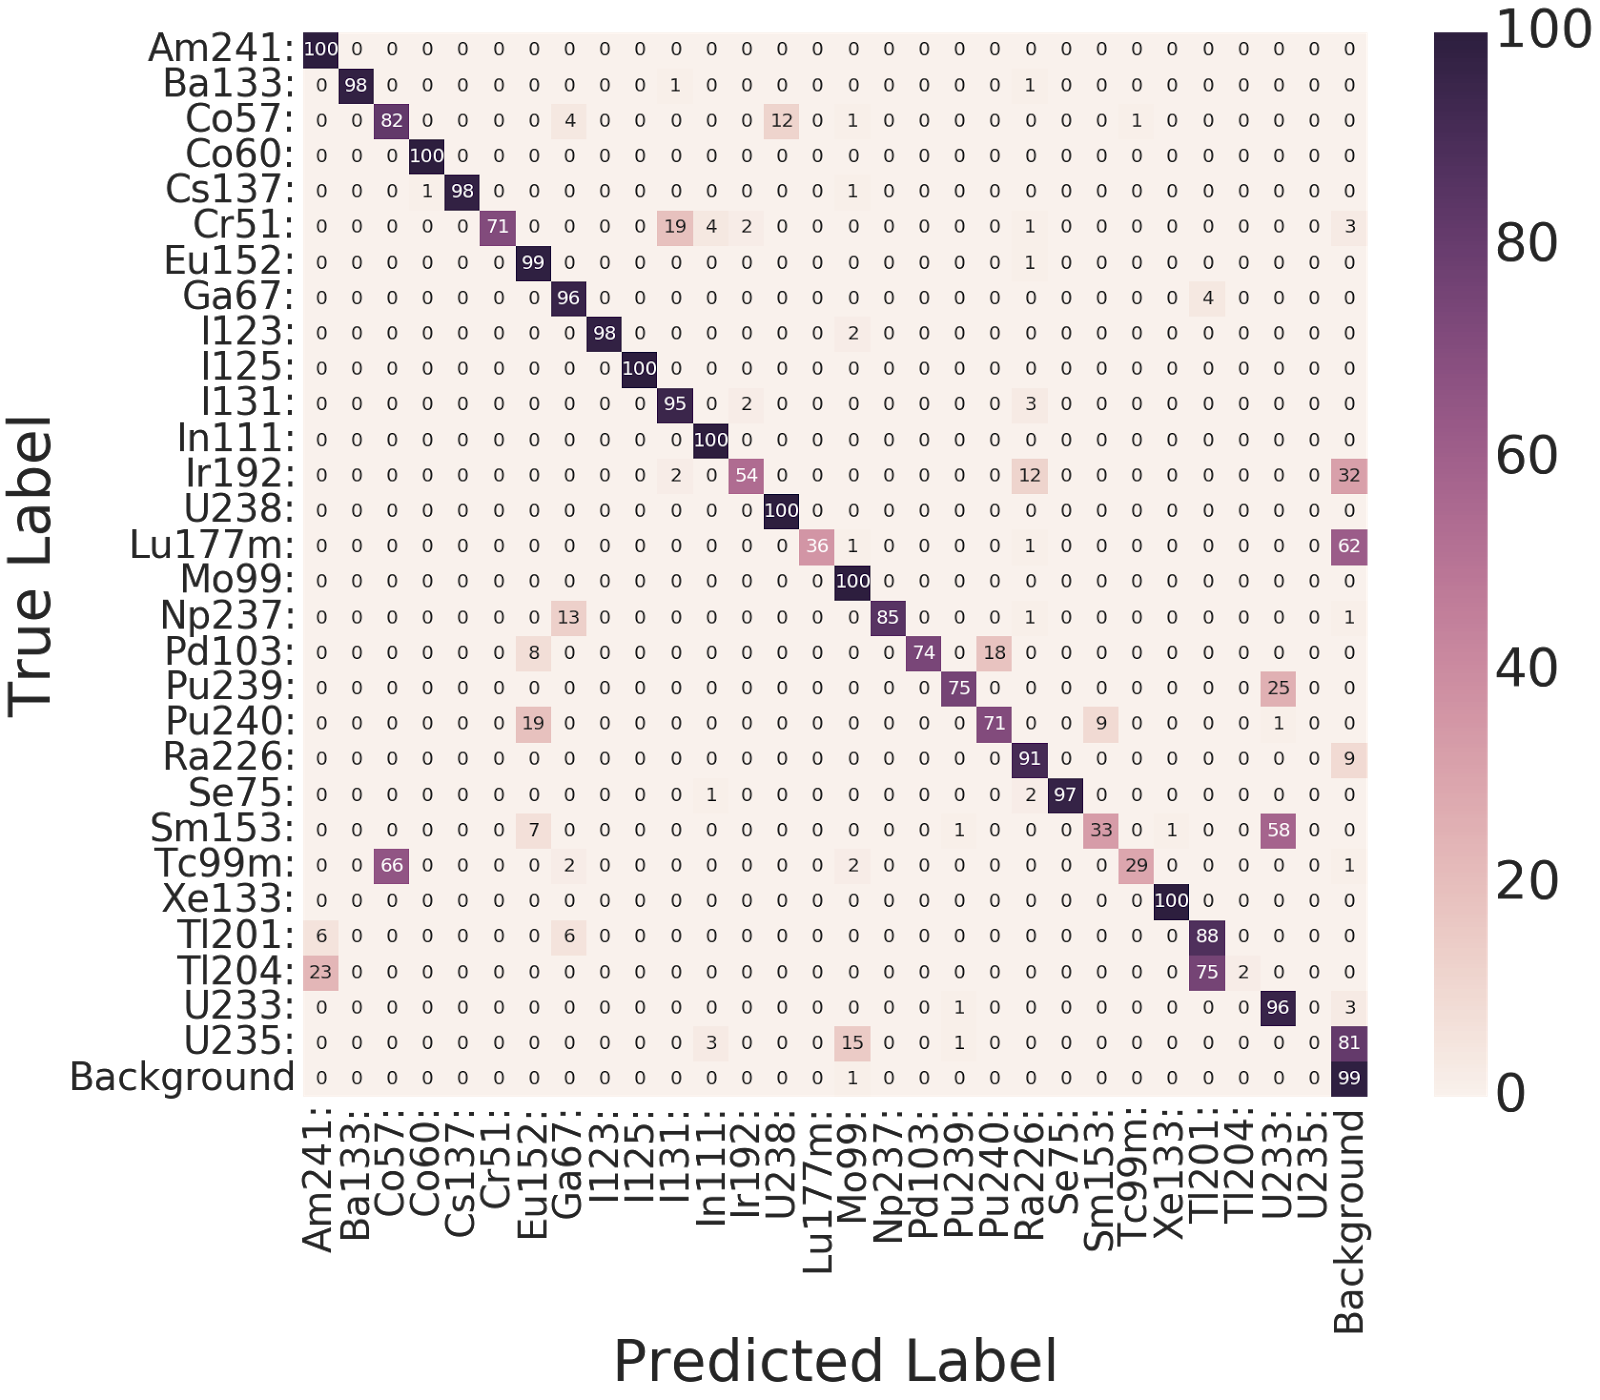
\includegraphics[width=\textwidth]{model_choice_hyperparameter_search_images/conf_matrix_example.png}
         \caption{Simple Training Dataset.}
         \label{fig:results_easy_distance_comparison_simple}
     \end{subfigure}
     \hfill
     \begin{subfigure}[b]{0.49\textwidth}
         \centering
         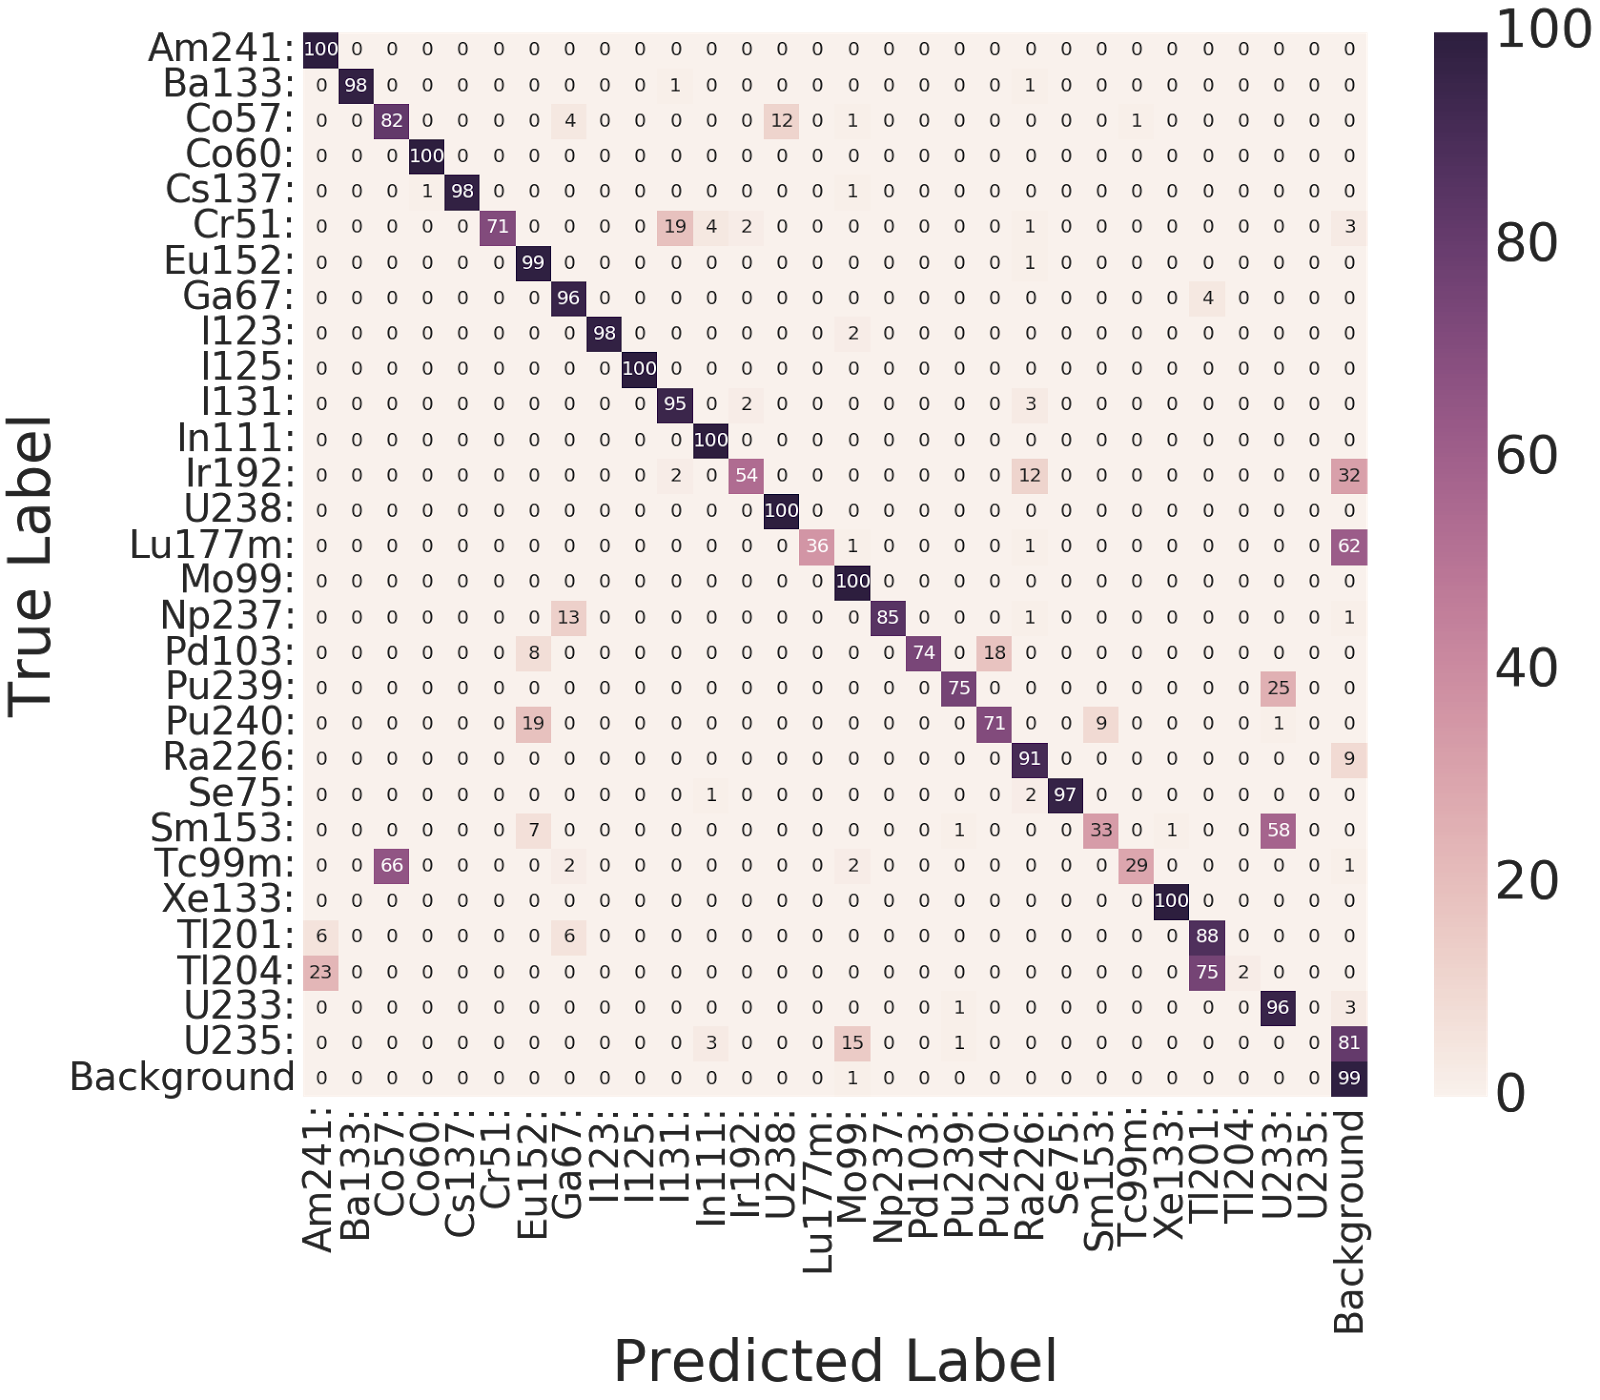
\includegraphics[width=\textwidth]{model_choice_hyperparameter_search_images/conf_matrix_example.png}
         \caption{Full Training Dataset.}
         \label{fig:results_easy_distance_comparison_full}
     \end{subfigure}
     
     \begin{subfigure}[b]{0.49\textwidth}
         \centering
         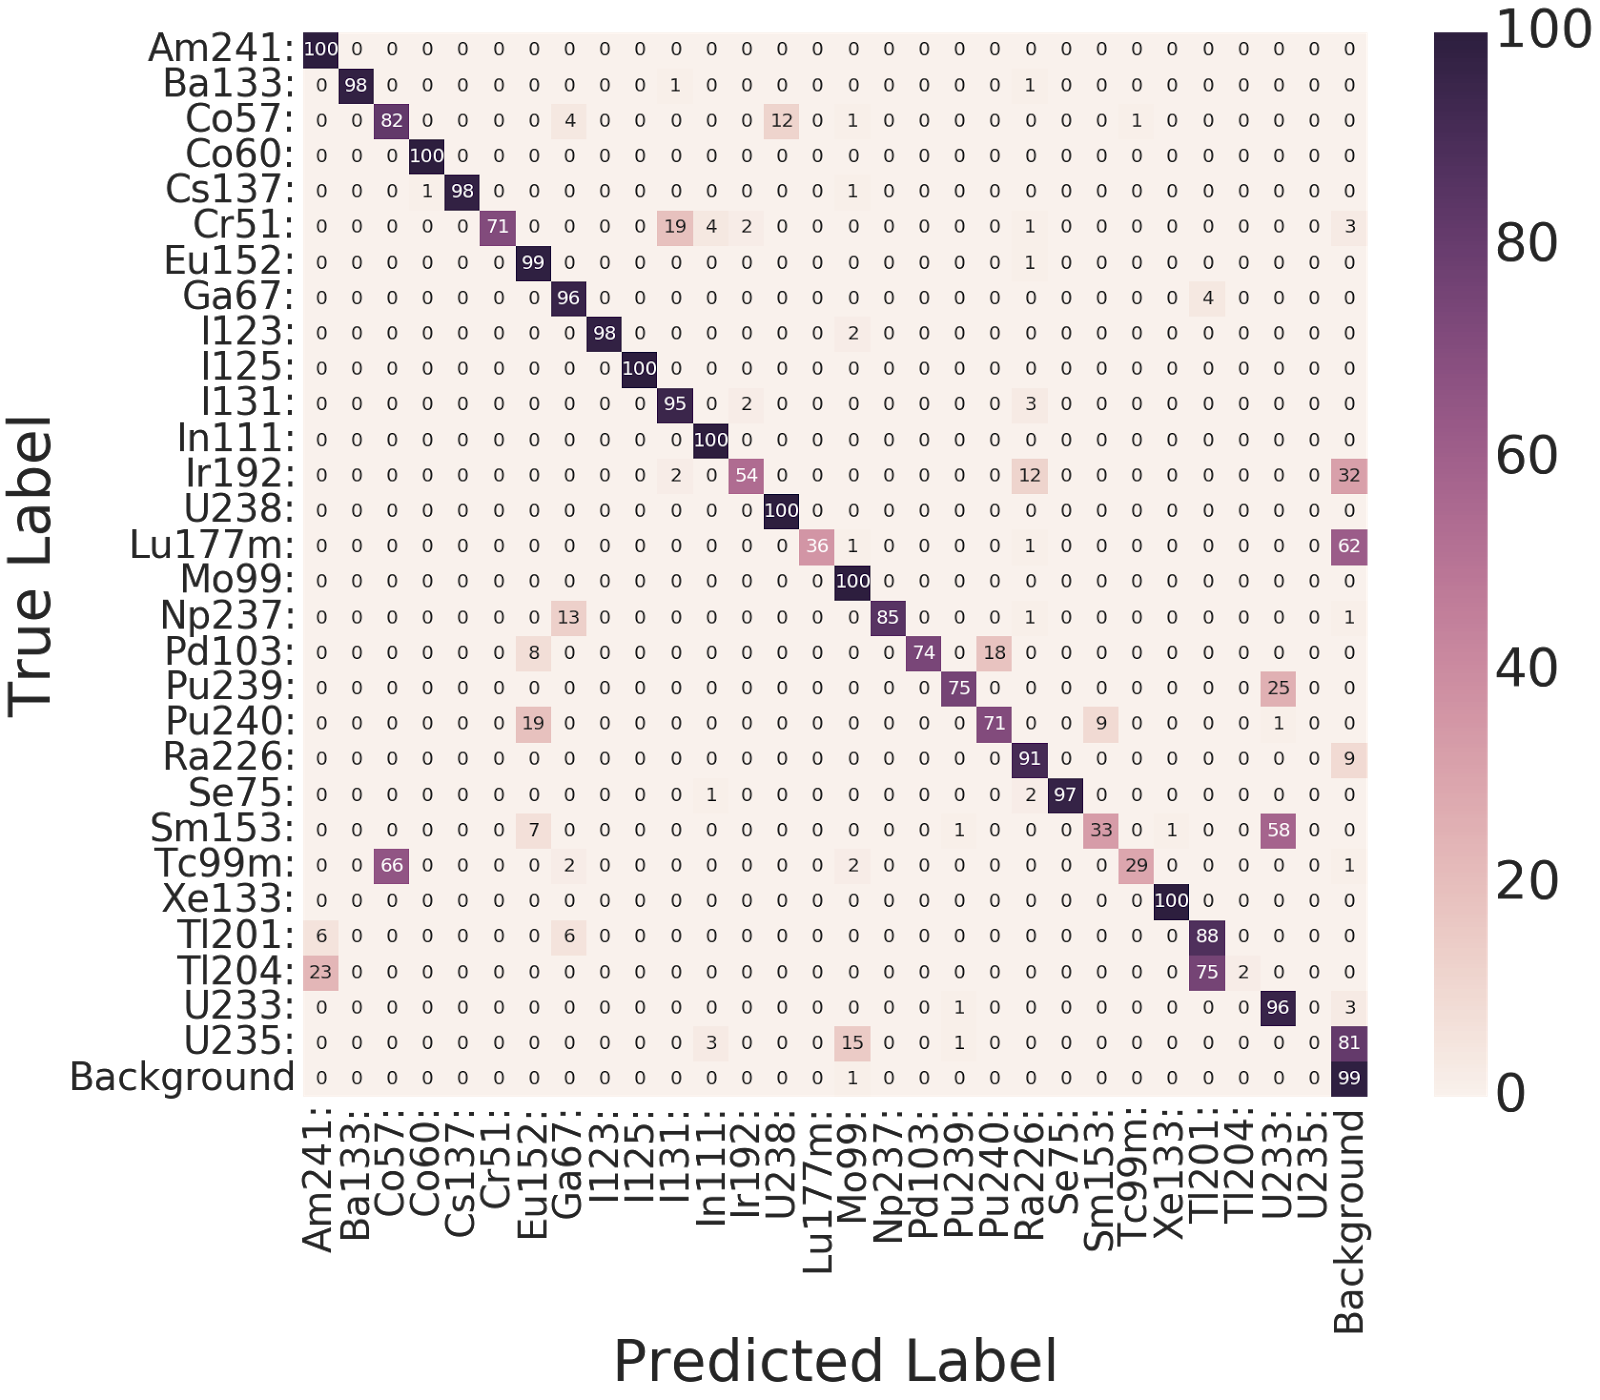
\includegraphics[width=\textwidth]{model_choice_hyperparameter_search_images/conf_matrix_example.png}
         \caption{Simple Training Dataset.}
         \label{fig:results_easy_distance_comparison_simple}
     \end{subfigure}
     \hfill
     \begin{subfigure}[b]{0.49\textwidth}
         \centering
         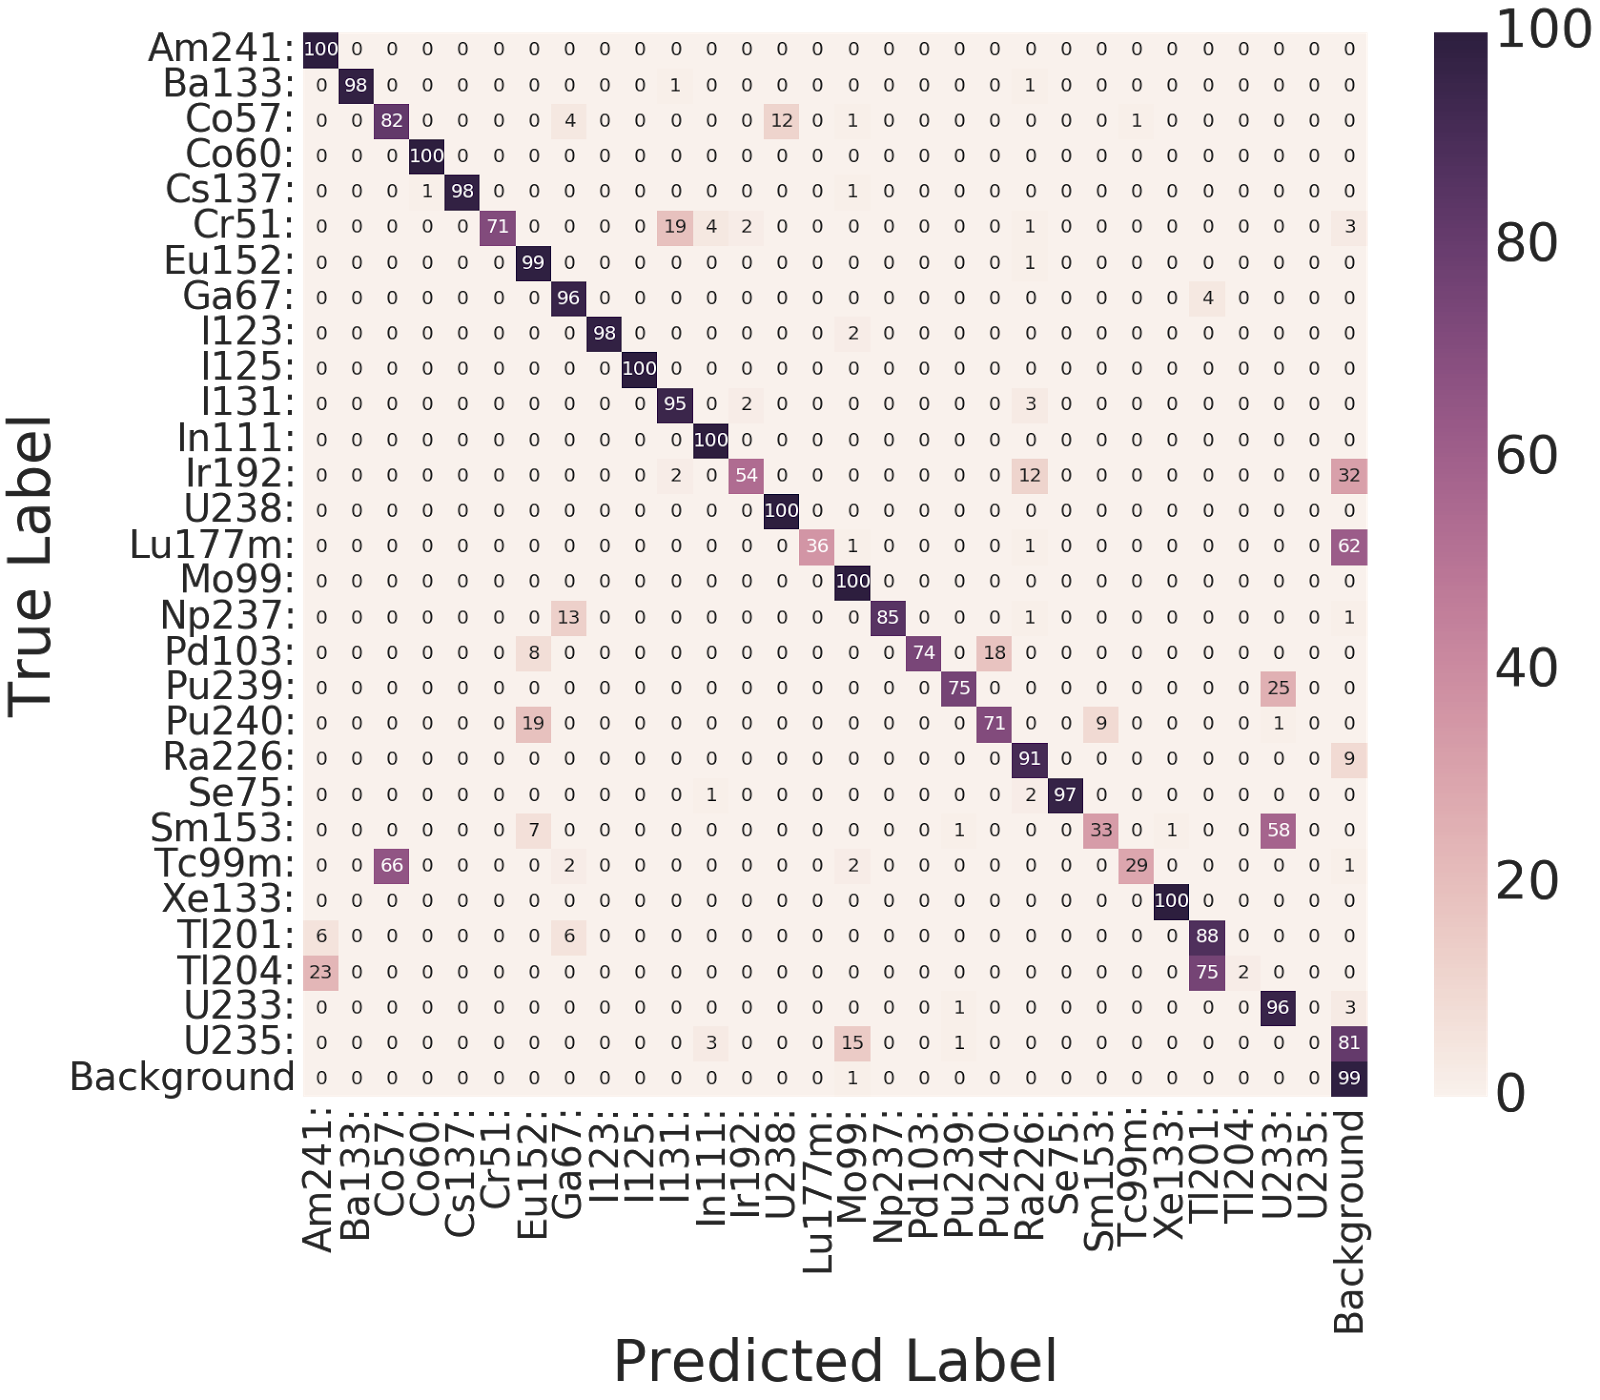
\includegraphics[width=\textwidth]{model_choice_hyperparameter_search_images/conf_matrix_example.png}
         \caption{Full Training Dataset.}
         \label{fig:results_easy_distance_comparison_full}
     \end{subfigure}
     
        \caption{Confusion matrices for the dataset with 60\% shielding.}
        \label{fig:results_easy_distance_comparison}
\end{figure}



\subsection{Generalization Dependence on Calibration.}

Datasets were simulated with various gain and offset setting.

\begin{figure}[H]
     \centering
     \begin{subfigure}[b]{0.9\textwidth}
         \centering
         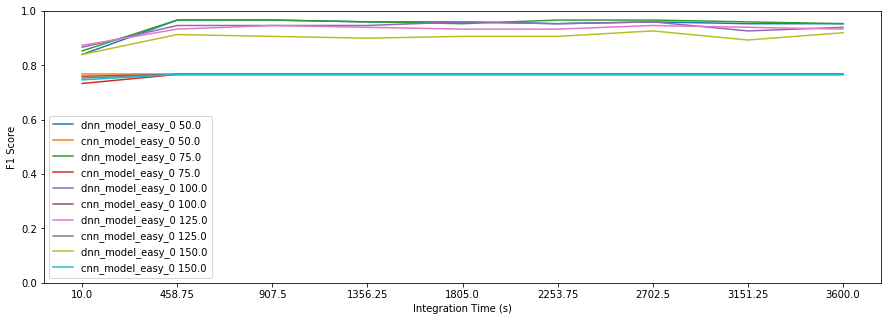
\includegraphics[width=\textwidth]{images/results_easy_distance_comparison}
         \caption{Simple Dataset.}
         \label{fig:results_easy_distance_comparison_simple}
     \end{subfigure}

     \begin{subfigure}[b]{0.9\textwidth}
         \centering
         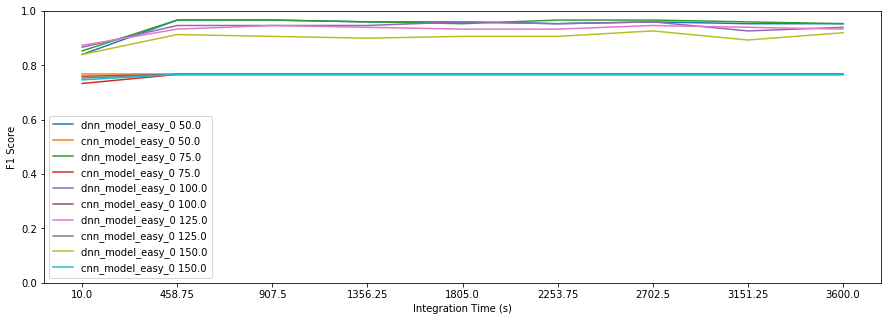
\includegraphics[width=\textwidth]{images/results_easy_distance_comparison}
         \caption{Full Dataset.}
         \label{fig:results_easy_distance_comparison_full}
     \end{subfigure}
        \caption{F1 score for all models trained on the simple dataset. Datasets included here used various gain and offset settings.}
        \label{fig:results_easy_distance_comparison}
\end{figure}



\subsection{Generalization Dependence on Changing Background.}

Datasets were simulated with backgrounds different from the training set and real measured background. It is expected that the full dataset will mistake background for isotopes more often than the simple dataset because photopeaks are decreased by shielding.


\begin{figure}[H]
     \centering
     \begin{subfigure}[b]{0.9\textwidth}
         \centering
         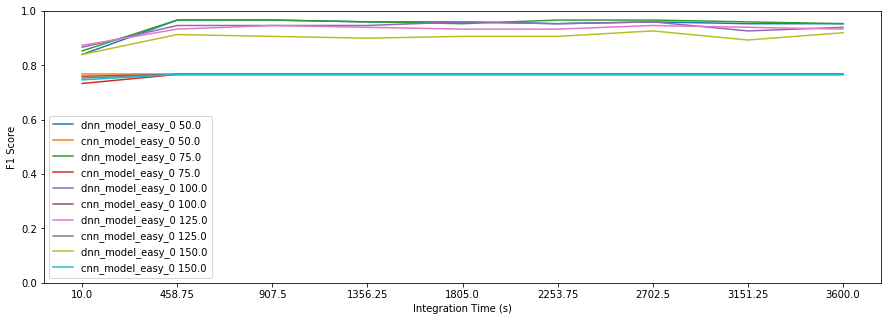
\includegraphics[width=\textwidth]{images/results_easy_distance_comparison}
         \caption{Simple Dataset.}
         \label{fig:fig:results_easy_background_simulated_simple}
     \end{subfigure}

     \begin{subfigure}[b]{0.9\textwidth}
         \centering
         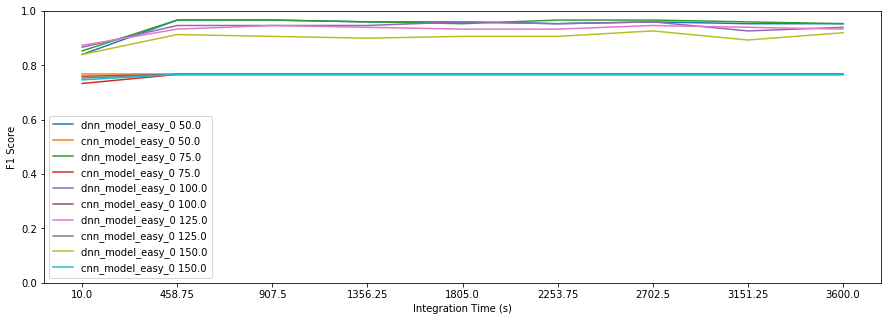
\includegraphics[width=\textwidth]{images/results_easy_distance_comparison}
         \caption{Full Dataset.}
         \label{fig:fig:results_easy_background_simulated_full}
     \end{subfigure}
        \caption{F1 score for all models trained on the simple dataset. Datasets included here used various amounts of shielding.}
        \label{fig:results_easy_background_simulated}
\end{figure}



Figure \ref{fig:results_full_background_inject} shows the identification performance on 

\begin{figure}[H]
     \centering
     \begin{subfigure}[b]{0.9\textwidth}
         \centering
         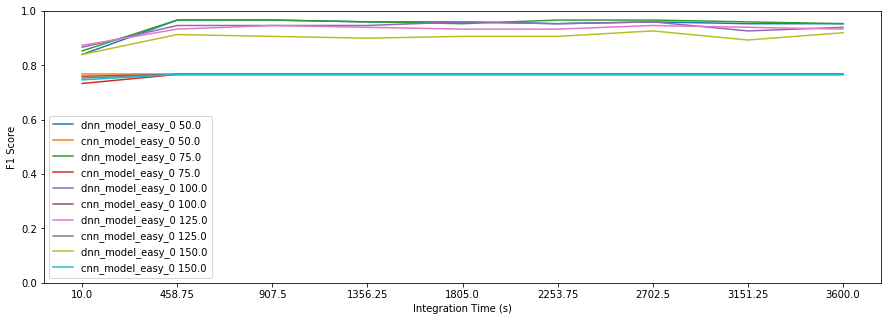
\includegraphics[width=\textwidth]{images/results_easy_distance_comparison}
         \caption{Simple Dataset.}
         \label{fig:results_full_background_inject_simple}
     \end{subfigure}

     \begin{subfigure}[b]{0.9\textwidth}
         \centering
         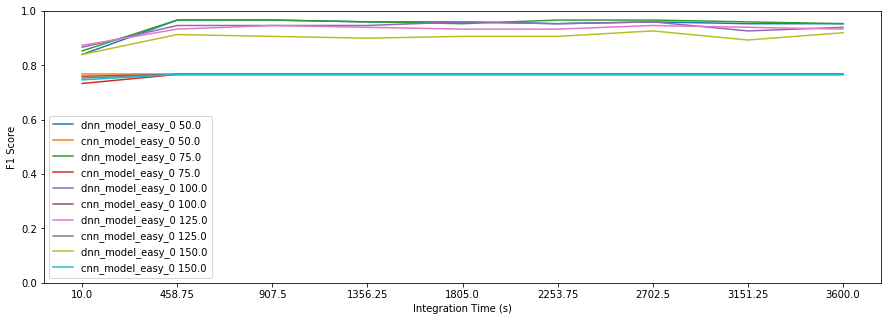
\includegraphics[width=\textwidth]{images/results_easy_distance_comparison}
         \caption{Full Dataset.}
         \label{fig:results_full_background_inject_full}
     \end{subfigure}
        \caption{F1 score for all models trained on the full dataset. Datasets included here used various amounts of shielding.}
        \label{fig:results_full_background_inject}
\end{figure}


% \section{Results from training all models}

% When training final models, two main questions need to be addressed: how good is a given architecture at solving a problem on its training dataset and how good is a given dataset at generalizing to outside examples.

% To determine how good a given architecture solves a problem, asymptotic convergence of the models performance needs to be measured. Because of the inherent stochastic nature of training machine learning algorithms (different random weight initialization, different mini-batches chosen during training, different data augmentation manifestations), each time a new network is trained the networks parameters and results will differ. This means a single trained instance of some model A may outperform a single trained instance of model B by chance, despite model B being an overall superior architecture. To more realistically compare how models perform on some dataset, a number of networks can be trained and their average performance compared. This is a method called bagging.

% \subsection{Asymptotic Model Performance on Training Dataset}

% For the best DNN and CNN architectures found in the hyperparameter search, using 'enough' data data samples as found in the hyperparameter search, 30 networks are trained. Their performance is observed in Figure \ref{fig:asymptotic_performance}.


%% Can also include performance using templates with extreme augmentation
% \begin{figure}[H]
% 	\centering
% 	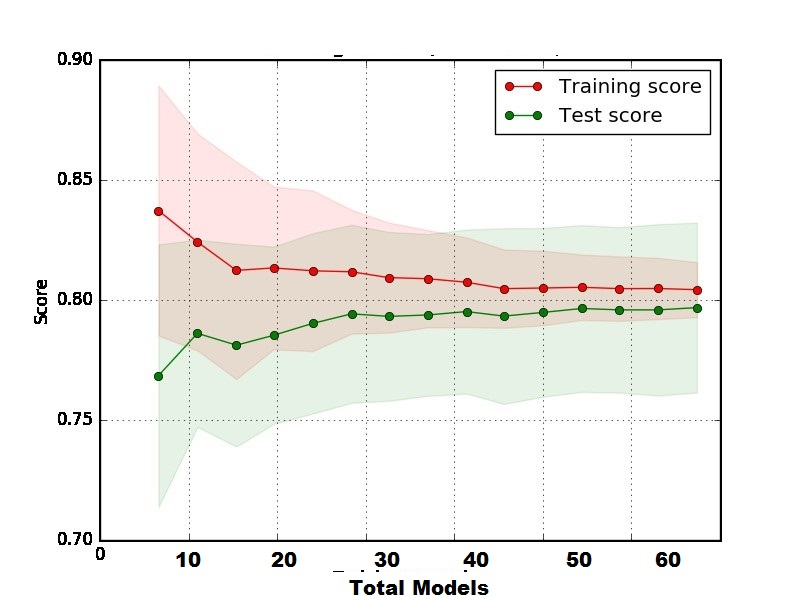
\includegraphics[width=0.8\linewidth]{model_choice_hyperparameter_search_images/asymptotic_performance_dummy}
% 	\caption{Asymptotic model performance for both the CNN and DNN on the training sets.}
% 	\label{fig:asymptotic_performance}
% \end{figure}

% Using N models as representative of asymptotic performance, justified in Figure \ref{fig:asymptotic_performance}, we can check out the confusion matrix associated with the test dataset to gain insight into how the algorithm is performing poorly and predict future shortcomings.


%% Can also include performance using templates with extreme augmentation
% \begin{figure}[H]
% 	\centering
% 	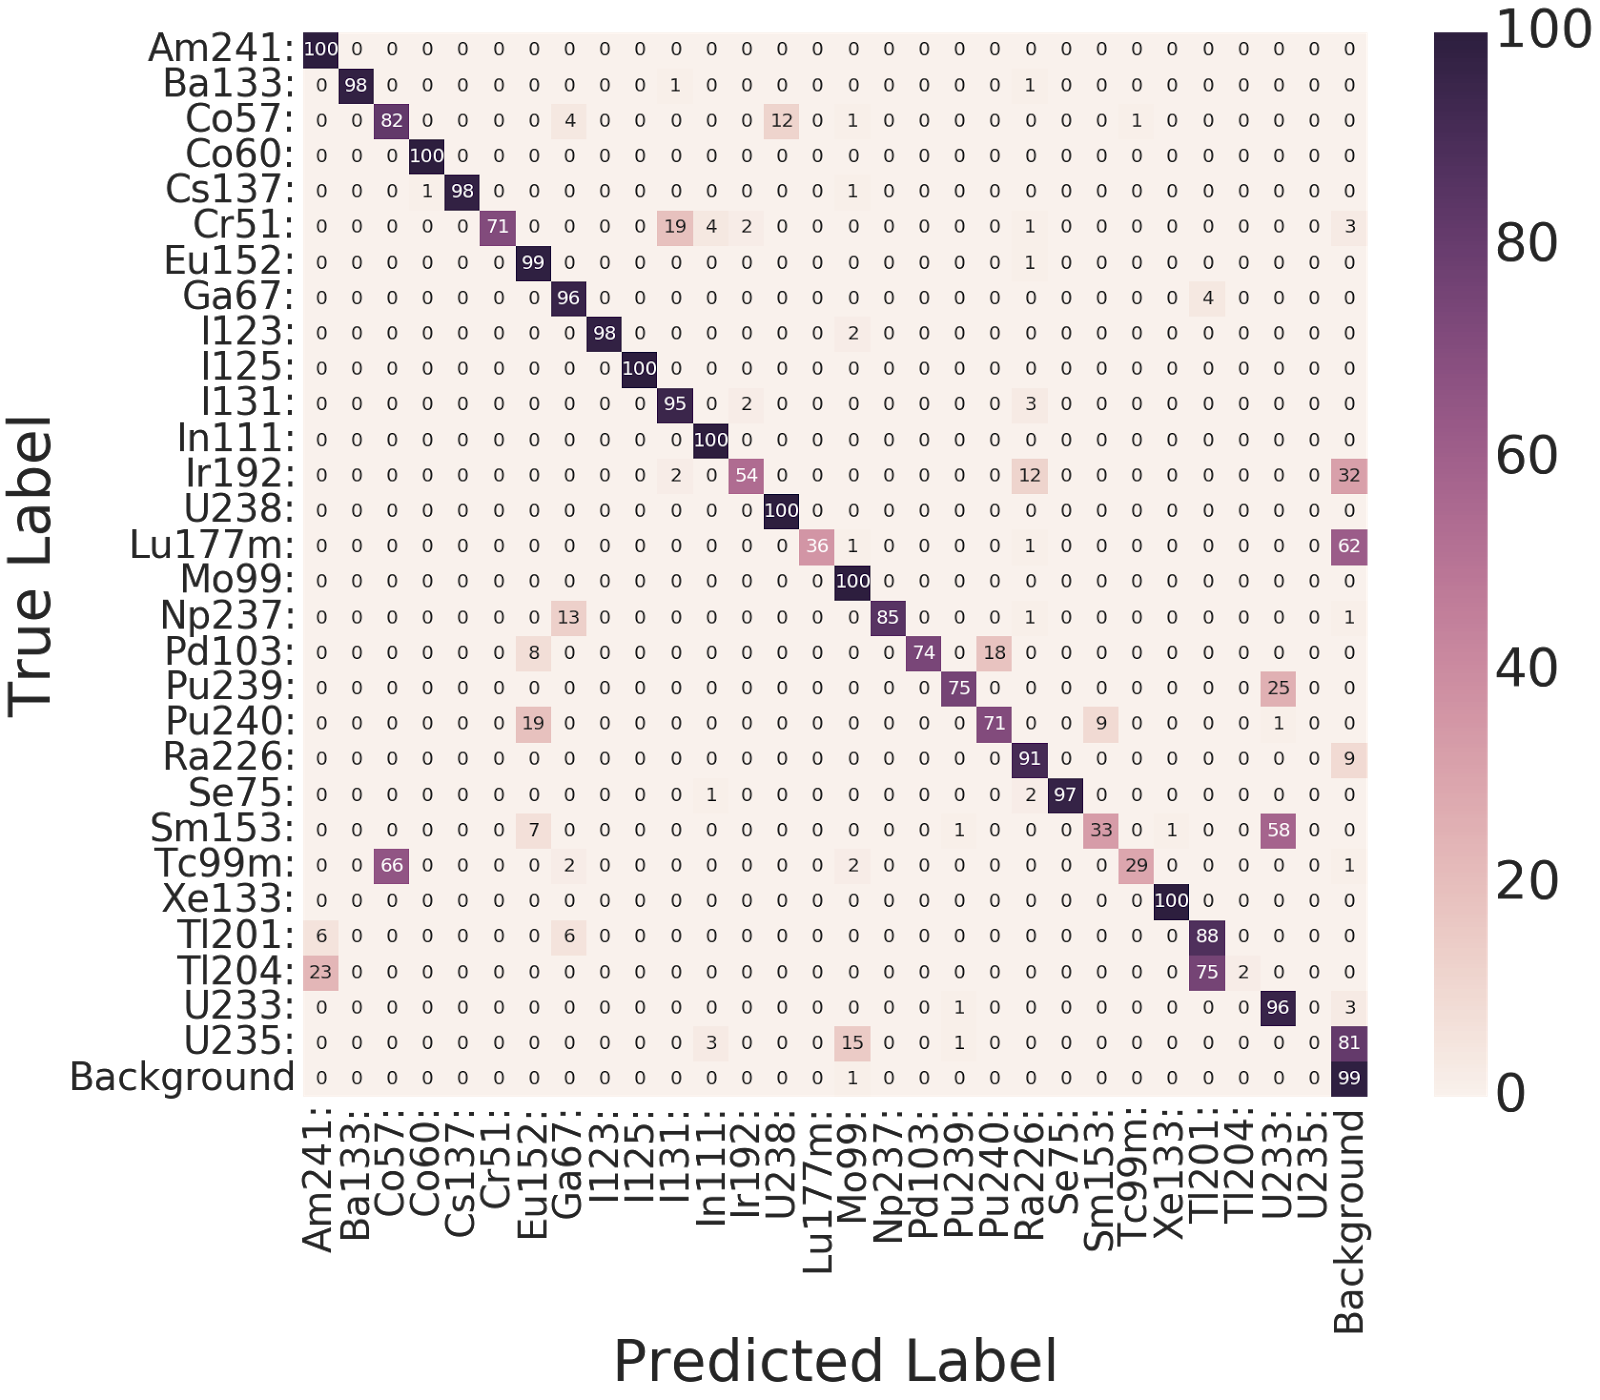
\includegraphics[width=0.8\linewidth]{model_choice_hyperparameter_search_images/conf_matrix_example}
% 	\caption{Asymptotic model performance for both the CNN and DNN on the training sets.}
% 	\label{fig:asymptotic_performance}
% \end{figure}

% Can also analyze how changing a threshold would affect precision/recall!

% \subsection{Results from training models using extreme data augmentation vs Data Augmentation grid sampling}

% Show learning curve between models 
% Instead of training examples on x-axis, plot against "number of divisions" (which also has a number of training examples included...)
% Note! You can start holding parameters constant to see what parameter the model is having difficulty explaining
% \begin{figure}[H]
%	\centering
%	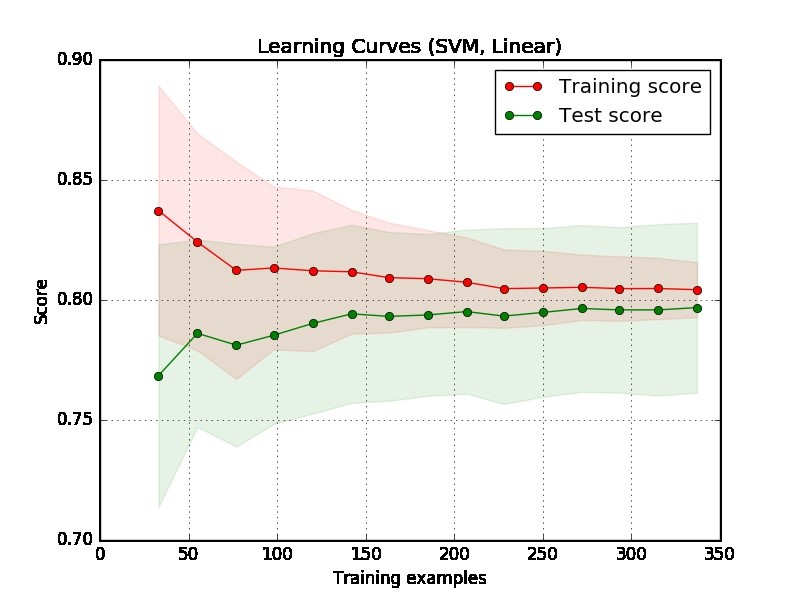
\includegraphics[width=0.8\linewidth]{model_choice_hyperparameter_search_images/learning_curve_dummy}
%	\caption{Learning curve example.}
%	\label{fig:Node}
%\end{figure}

%% Plot of average F1-score vs epochs for all models. Datasets include different detector model (use this as validation set) and same detector model with certain augmentation parameters frozen (or just the training set).


%% Plot of average F1-score vs epochs for all models. Datasets include different detector model (us this as validation set) and same detector model with certain augmentation parameters frozen (or just the training set).

\subsection{Results on Spectra for ANSI compliance}

This section shows model asymptotic performance vs integration time for ANSI compliance. Using N models (justified previously as asymptotic). 



\begin{table}[H]
\centering
\caption{Isotope combinations required for the ANSI standard \cite{ANSI}.}
\begin{tabular}{c}
Isotope Combinations \\ \hline
$^{137}$Cs + depleted uranium (DU) \\ % \hline
$^{99m}$Tc + HEU \\ % \hline
$^{201}$Tl + HEU \\ % \hline
$^{67}$Ga + HEU \\ % \hline
$^{131}$I + WGPu \\ % \hline
NORM + HEU \\ % \hline
NORM + WGPu \\ % \hline
\end{tabular}
\end{table}



\begin{figure}[H]
     \centering
     \begin{subfigure}[b]{0.9\textwidth}
         \centering
         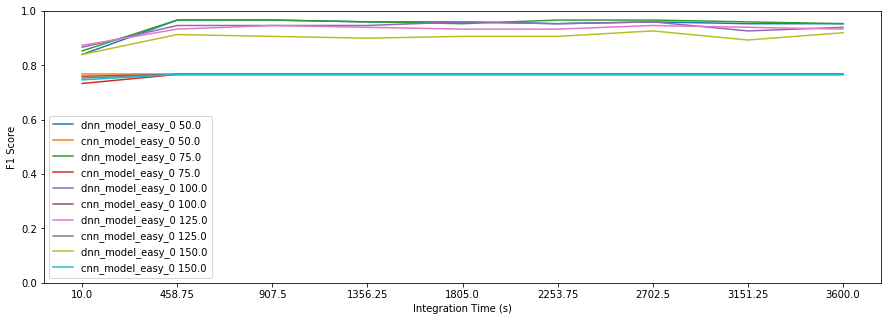
\includegraphics[width=\textwidth]{images/results_easy_distance_comparison}
         \caption{Simple Dataset.}
         \label{fig:results_full_background_inject_simple}
     \end{subfigure}

     \begin{subfigure}[b]{0.9\textwidth}
         \centering
         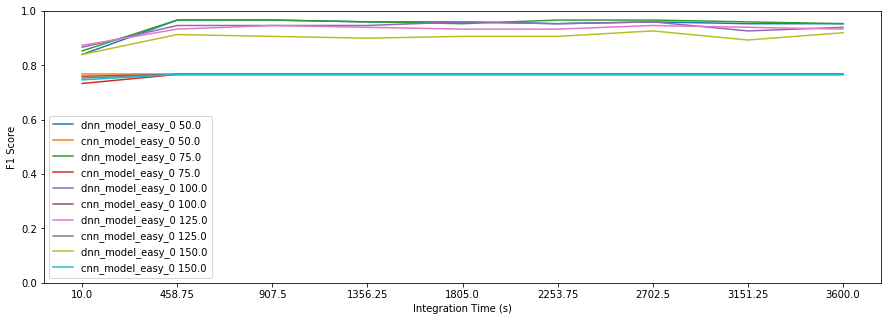
\includegraphics[width=\textwidth]{images/results_easy_distance_comparison}
         \caption{Full Dataset.}
         \label{fig:results_full_background_inject_full}
     \end{subfigure}

        \caption{F1 score for models tested on ANSI isotope combinations.}
        \label{fig:results_full_background_inject}
\end{figure}



\subsection{Results on Measured Spectra}

This section shows model asymptotic performance vs integration time for a few different settings (different voltages, shielding)

To investigate how each model identified real spectra behind shielding and spectra with different calibrations, real spectra were measured. Sources include $^{137}$Cs, $^{60}$Co, $^{133}$Ba, and $^{152}$Eu. 


\subsubsection{Asymptotic Model Performance on Changing Voltage}

To see the generalization performance of the model to changing calibration, spectra with different voltages are recorded and their asymptotic performance compared.

Spectra were measured with different detector calibrations. A 2x2 Ortec NaI detector was set to 770 V, setting it's 1024th channel to 3 MeV. To capture a large range of calibrations, voltages varied from 720 V to 820 V in steps of 15 V. The $^{137}$Cs, $^{60}$Co, and $^{133}$Ba source had an activity of 1$\mu$C. For these sources, a source-to-detector distance of 14.25 mm was used to keep the cps on the detector from the source equal to the cps on the detector from background.

Figures \ref{fig:model_asymptotic_performance_co60} and \ref{fig:model_asymptotic_performance_cs137} show performance for isotopes with comparatively simple spectra.


\begin{figure}[H]
     \centering
     \begin{subfigure}[b]{0.9\textwidth}
         \centering
         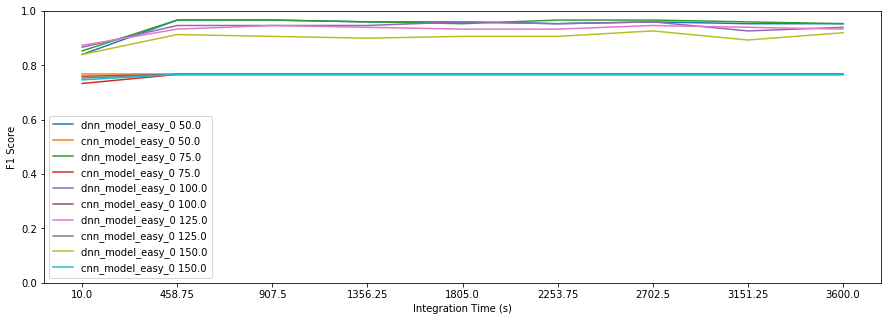
\includegraphics[width=\textwidth]{images/results_easy_distance_comparison}
         \caption{$^{60}$Co}
         \label{fig:model_asymptotic_performance_co60}
     \end{subfigure}

     \begin{subfigure}[b]{0.9\textwidth}
         \centering
         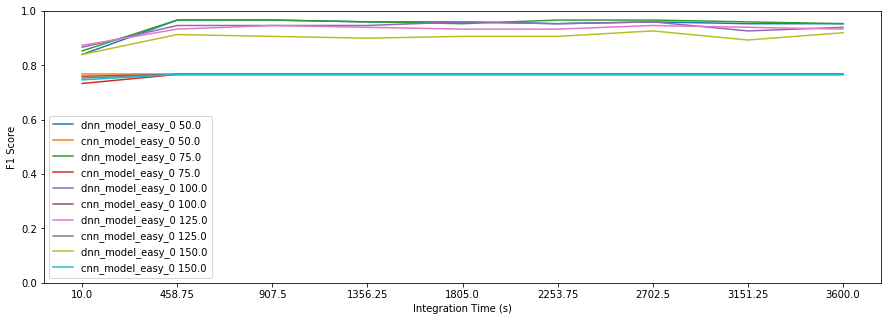
\includegraphics[width=\textwidth]{images/results_easy_distance_comparison}
         \caption{$^{137}$Cs.}
         \label{fig:results_easy_distance_comparison_full}
     \end{subfigure}
     
     \begin{subfigure}[b]{0.9\textwidth}
         \centering
         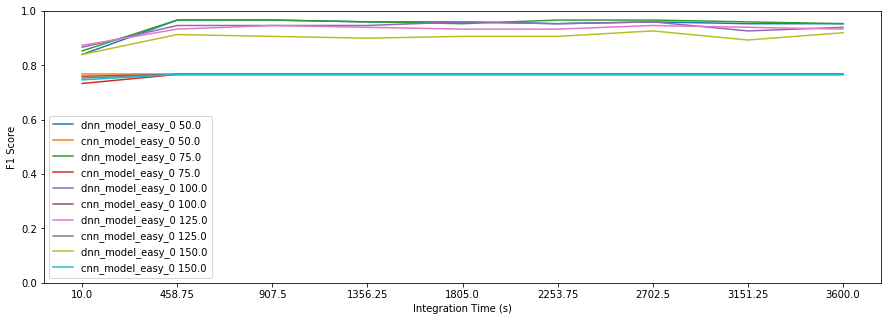
\includegraphics[width=\textwidth]{images/results_easy_distance_comparison}
         \caption{$^{152}$Eu.}
         \label{fig:results_easy_distance_comparison_full}
     \end{subfigure}
     
     \begin{subfigure}[b]{0.9\textwidth}
         \centering
         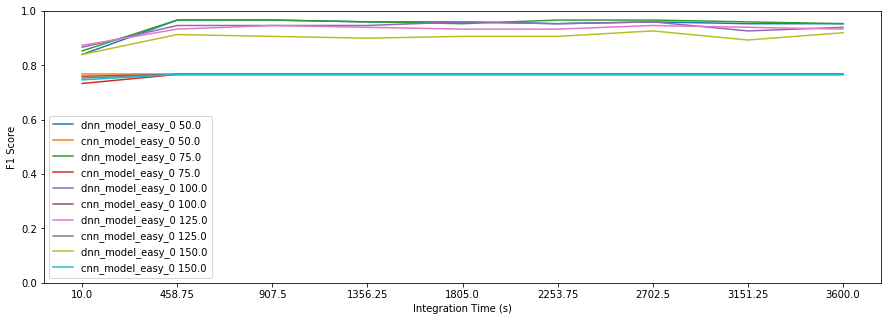
\includegraphics[width=\textwidth]{images/results_easy_distance_comparison}
         \caption{$^{133}$Ba.}
         \label{fig:results_easy_distance_comparison_full}
     \end{subfigure}

        \caption{F1 score for all models trained on the simple dataset. Spectra measured with different gain settings.}
        \label{fig:results_easy_distance_comparison}
\end{figure}


\begin{figure}[H]
     \centering
     \begin{subfigure}[b]{0.9\textwidth}
         \centering
         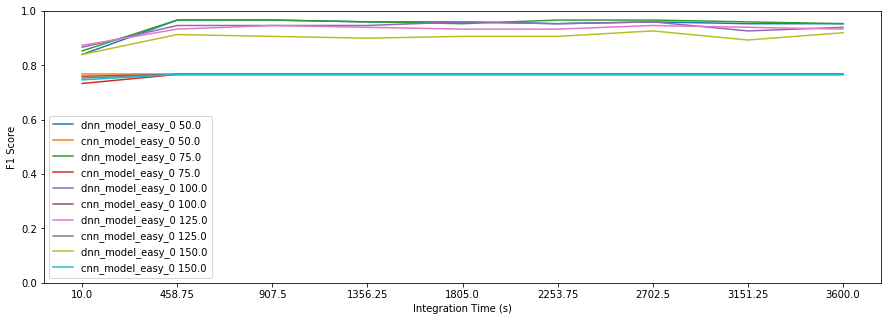
\includegraphics[width=\textwidth]{images/results_easy_distance_comparison}
         \caption{$^{60}$Co}
         \label{fig:model_asymptotic_performance_co60}
     \end{subfigure}

     \begin{subfigure}[b]{0.9\textwidth}
         \centering
         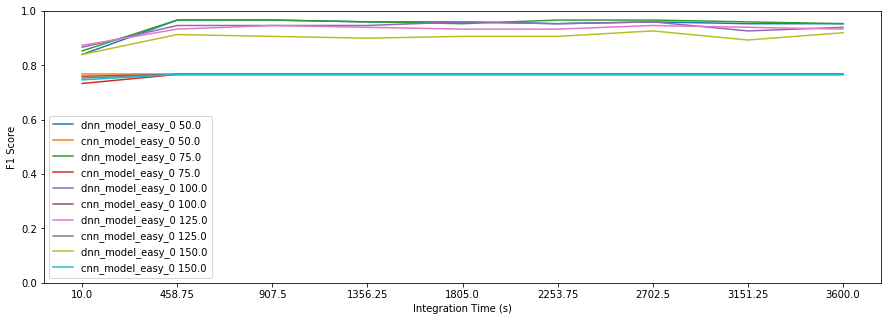
\includegraphics[width=\textwidth]{images/results_easy_distance_comparison}
         \caption{$^{137}$Cs.}
         \label{fig:results_easy_distance_comparison_full}
     \end{subfigure}
     
     \begin{subfigure}[b]{0.9\textwidth}
         \centering
         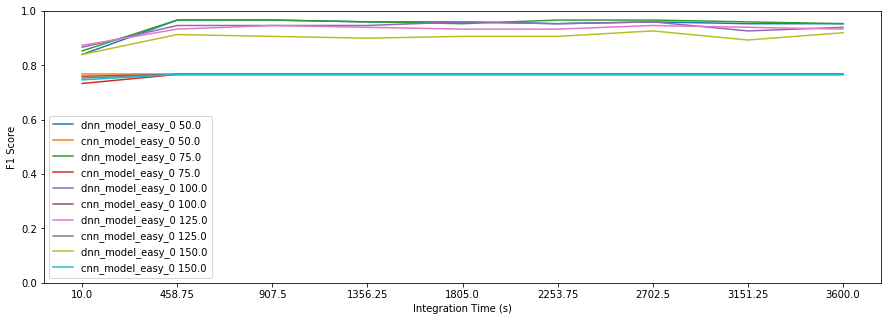
\includegraphics[width=\textwidth]{images/results_easy_distance_comparison}
         \caption{$^{152}$Eu.}
         \label{fig:results_easy_distance_comparison_full}
     \end{subfigure}
     
     \begin{subfigure}[b]{0.9\textwidth}
         \centering
         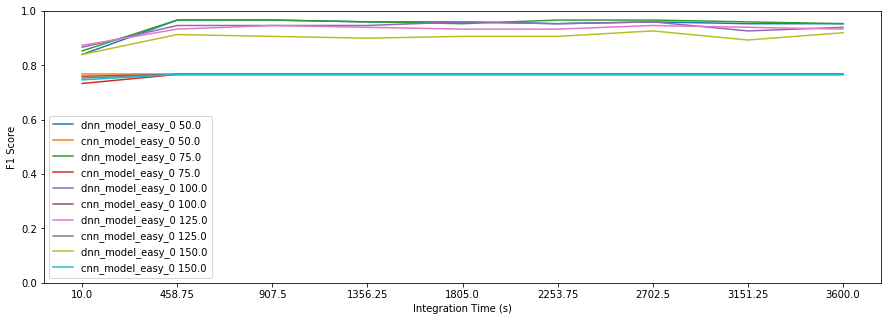
\includegraphics[width=\textwidth]{images/results_easy_distance_comparison}
         \caption{$^{133}$Ba.}
         \label{fig:results_easy_distance_comparison_full}
     \end{subfigure}

        \caption{F1 score for all models trained on the full dataset. Spectra measured with different gain settings.}
        \label{fig:results_easy_distance_comparison}
\end{figure}


